\cia
\subsection{Multipole Truncation Results for $R_{EM}$ and $R_{SM}$}
The result for the ratios $R_{EM}$ and $R_{SM}$ are shown in Table 
\ref{tab:result_ratio} for different values of $Q^2$.

The fits suggest a zero crossing for $R_{EM}$ between $Q^2$ of $3.0$ and $4.0$ GeV$^2$.

\begin{table}[h]
 \begin{center}
  \begin{tabular}{c | c | c}
          & & \\
    \hline\hline    
        & & \\
    $Q^2$ (GeV$^2$)&     $R_{EM}$ ($\%, E_{STAT},E_{SYS}$)   &    $R_{SM}$ ($\%, E_{STAT},E_{SYS}$) \\ 
    & & \\
    \hline\hline
        & & \\

     
2.15  & $  -1.0 \pm 0.7 \pm 0.05  $  &  $ -10.0  \pm 0.9 \pm 0.06 $ \\
2.4   & $  0.4  \pm 0.3 \pm 0.2   $  &  $ -11.7  \pm 0.5 \pm 0.2  $ \\
3     & $  1.3  \pm 0.4 \pm 0.3   $  &  $ -12.5  \pm 0.5 \pm 0.07 $ \\
3.5   & $  1.2  \pm 0.5 \pm 0.3   $  &  $ -12.9  \pm 0.7 \pm 0.2  $ \\
4.2   & $  1.7  \pm 0.6 \pm 0.4   $  &  $ -17.3  \pm 1.0 \pm 0.14 $ \\
5     & $  6.0  \pm 1.0 \pm 0.5   $  &  $ -24.0  \pm 1.8 \pm 0.24 $ \\
6     & $  4.8  \pm 1.8 \pm 0.7   $  &  $ -24.0  \pm 4   \pm 0.4  $ \\
& & \\
    \hline
  \end{tabular}
 \end{center} 
 \caption{ Results for $R_{EM}$ and $R_{SM}$ in the multipole truncation analysis.}
 \label{tab:result_ratio}
\end{table}

$R_{EM}$ is shown in \F{fig:RM} along with the prediction from DMT 2001 and MAID 2000 models.
Previous data from CLAS and Hall C (using  $M_{1+}$ dominance and $\ell \le 1$ approximations) 
are also plotted.


\begin{figure}[h]
 \begin{center}
 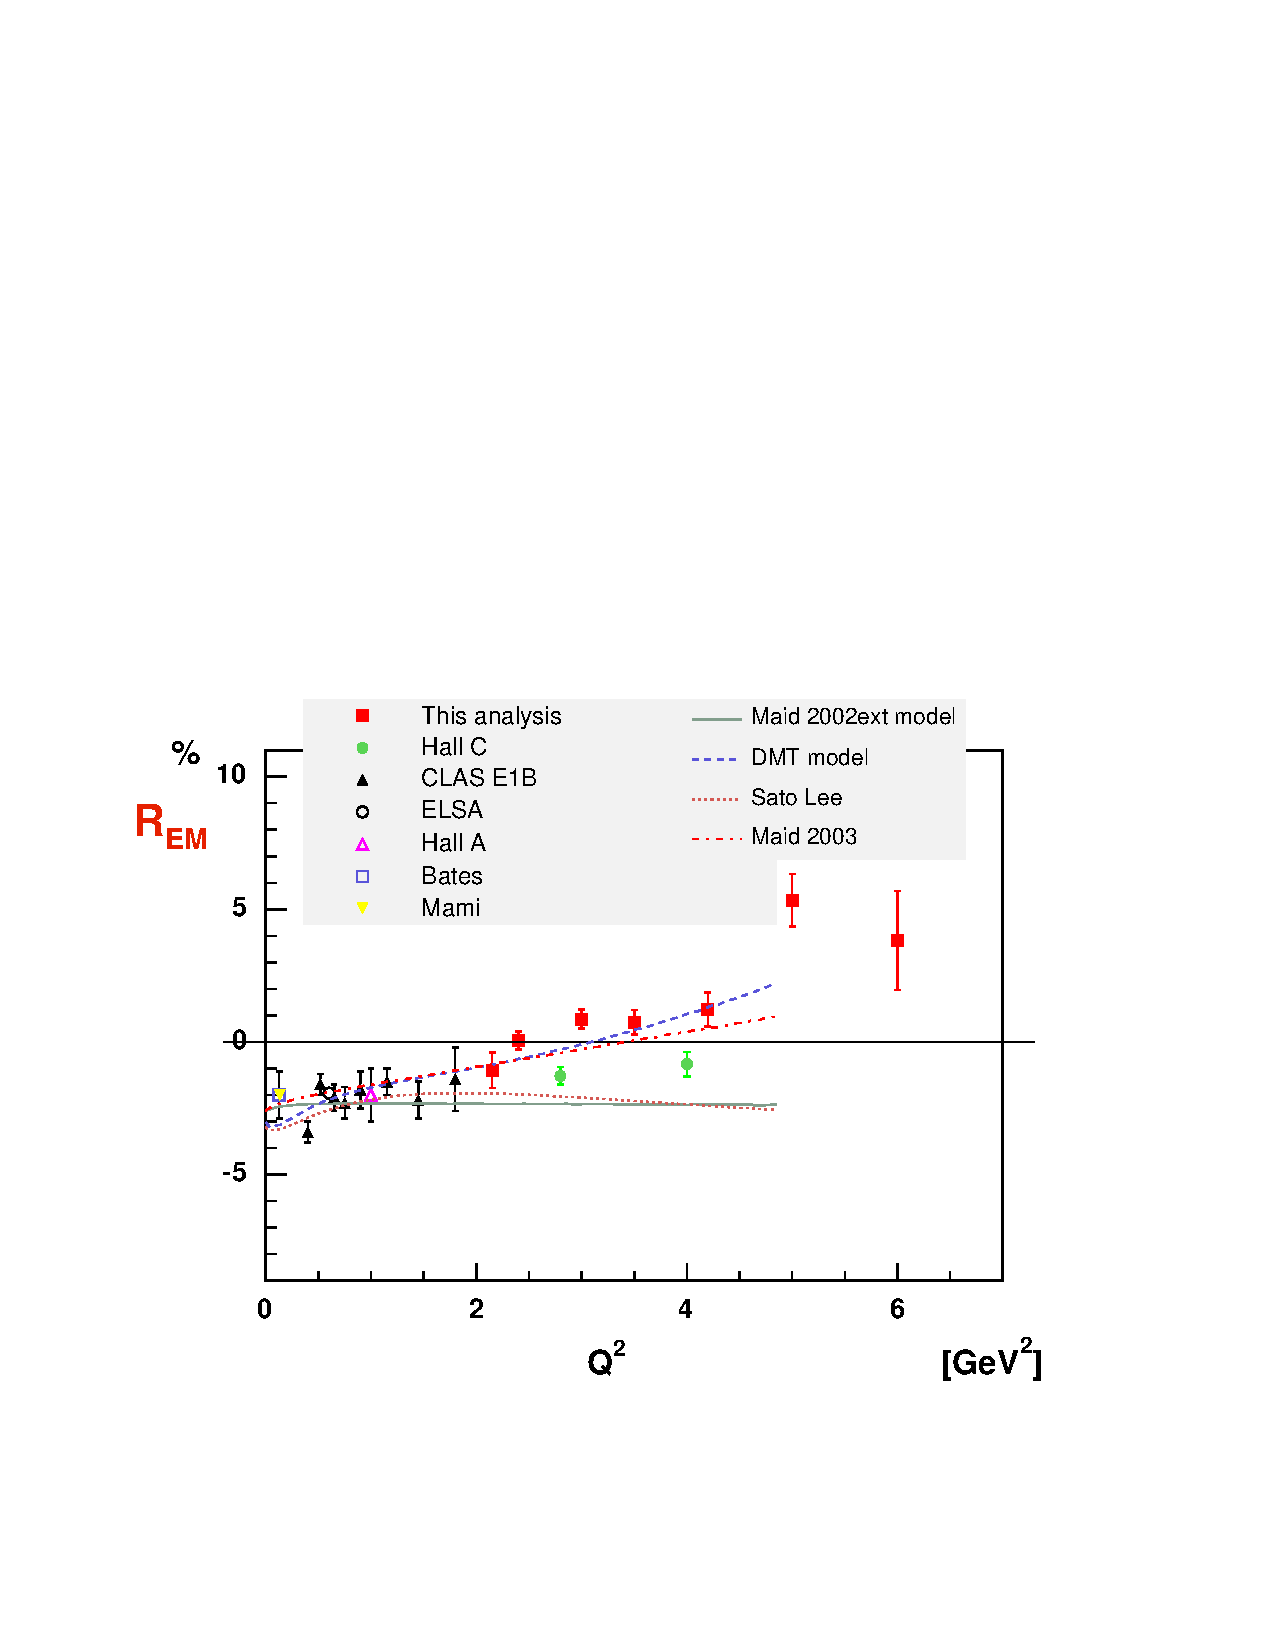
\includegraphics[width = 11cm, bb=30 130 520 500]{analysis/img/RM} 
  \caption[Result for $R_{EM}$ as a function of $Q^2$]
          {  Result for $R_{EM}$ as a function of $Q^2$ obtained in the $M_{1+}$ dominance approximation.}
 \label{fig:RM}
\end{center}
\end{figure}


\begin{figure}[h]
 \begin{center}
 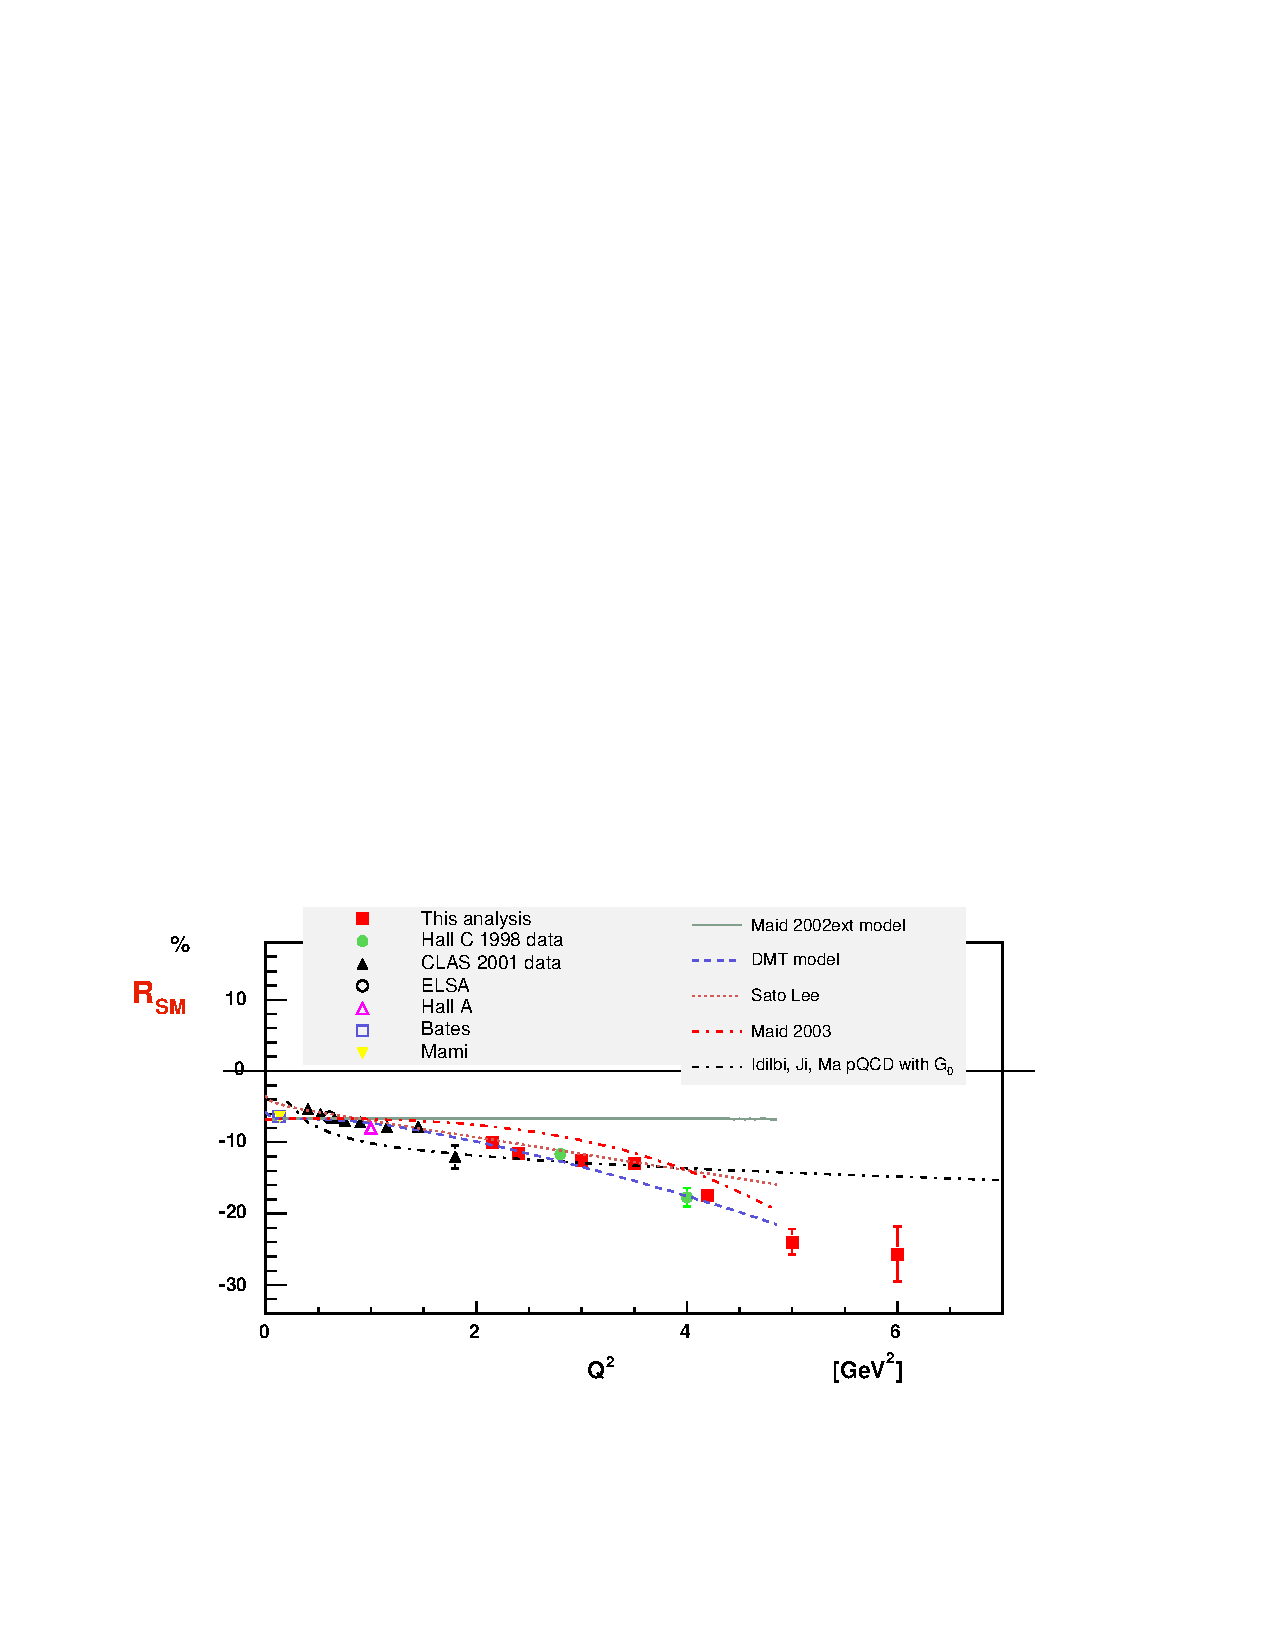
\includegraphics[width = 11cm, bb=30 130 520 500]{analysis/img/RS} 
  \caption[Result for $R_{SM}$ as a function of $Q^2$]
          {  Result for $R_{SM}$ as a function of $Q^2$ obtained in the $M_{1+}$ dominance approximation.}
 \label{fig:SM}
\end{center}
\end{figure}

\cia
\subsection{Amplitudes of $M_{1-}$, $E_{0+}$, $S_{0+}$}
Equations  (\ref{eqno:m1dominance}) holds if $|M_{1+}| >> |M_{\ell\pm}|$ where $ M_{\ell\pm}$ is any 
e.m. multipole that can contribute to the process. The extraction of $M_{1-}$, $E_{0+}$ and $S_{0+}$
using (\ref{eqno:m1dominance}) is a consistency check of the  $M_{1+}$ dominance assumption.
In \F{fig:M1m} and \F{fig:E0p} it is shown the result of the ratios  Re$(M_{1-}^*M_{1+})/|M_{1+}|^2$, 
Re$(E_{0+}^*M_{1+})/|M_{1+}|^2$ and Re$(S_{0+}^*M_{1+})/|M_{1+}|^2$. These amplitudes are 
about $10-20 \% $ of in $|M_{1+}|$ amplitude, increasing with $Q^2$. This rather large result suggest that   
Equations  (\ref{eqno:m1dominance}) are only approximate.

\begin{figure}[h]
 \begin{center}
 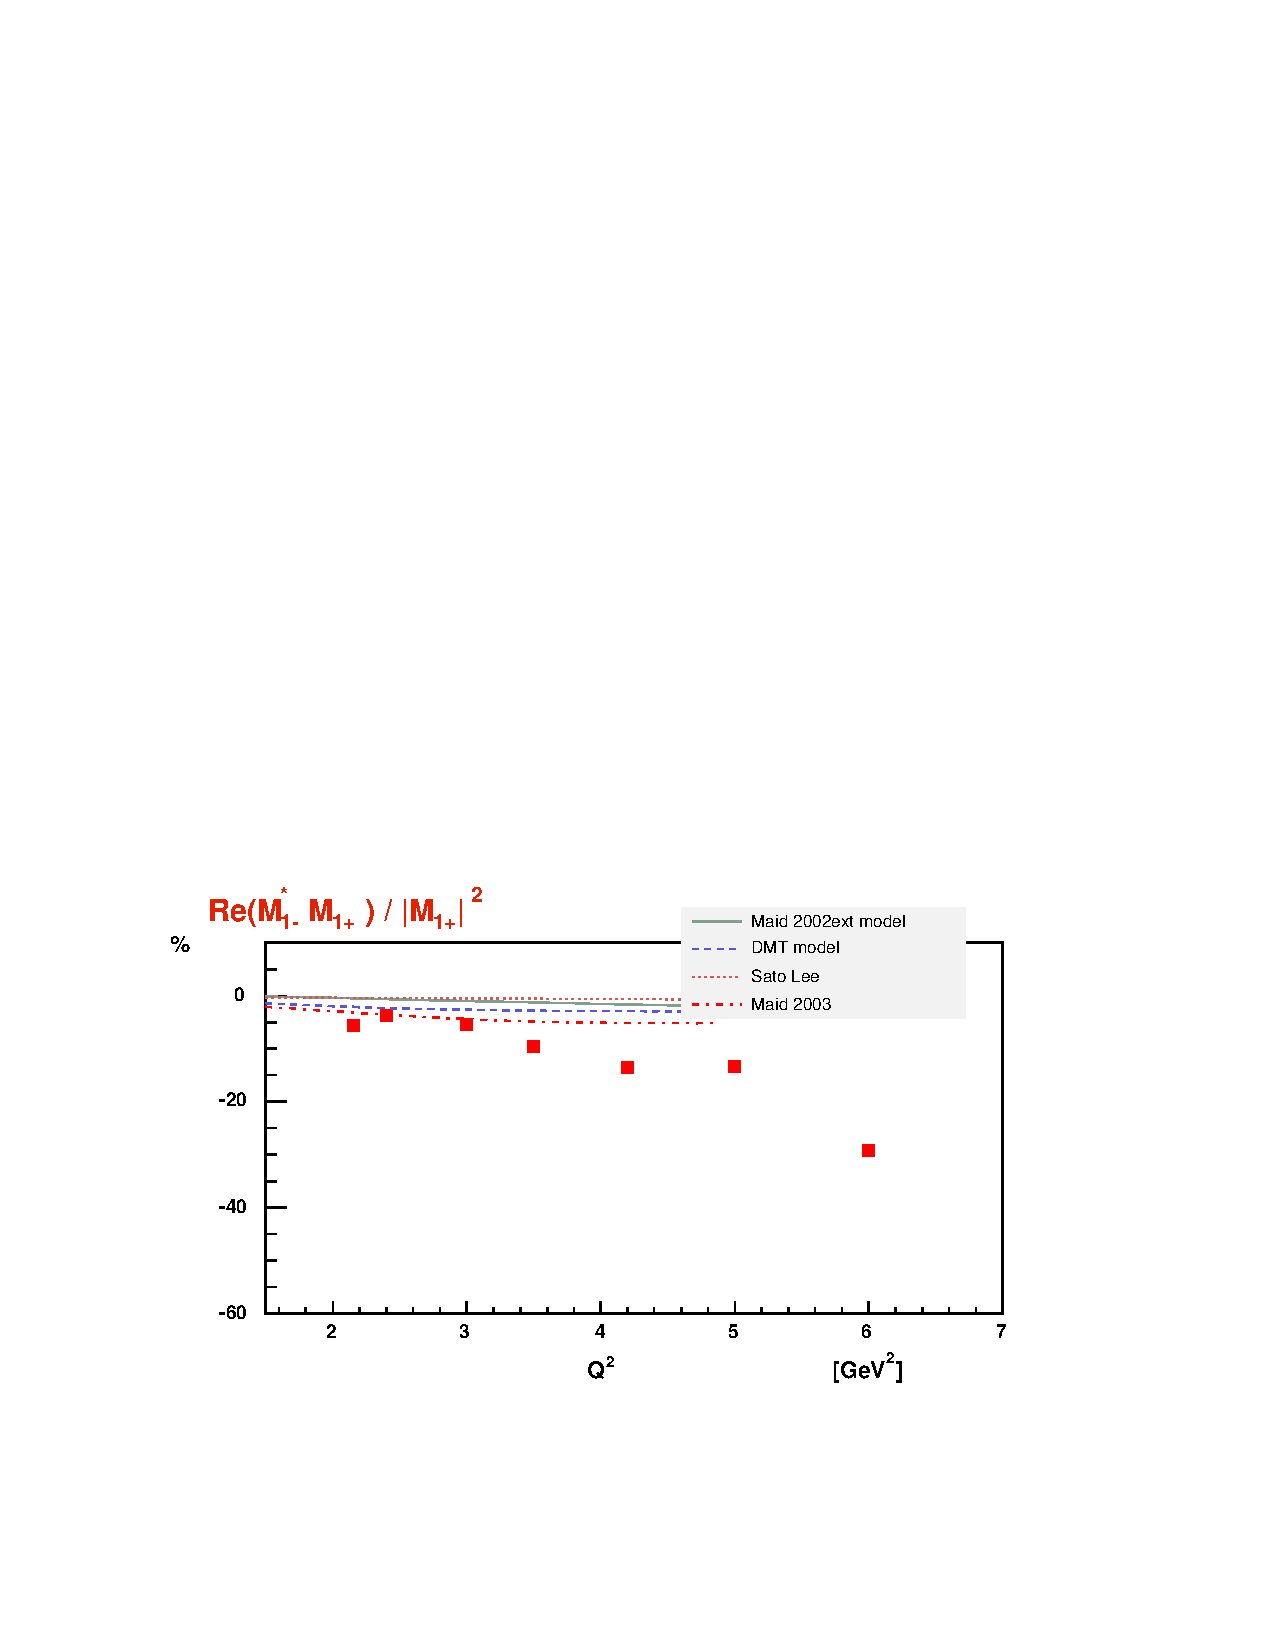
\includegraphics[width = 11cm, bb=30 120 520 400]{analysis/img/M1m} 
  \caption[Amplitude of $M_{1-}$]
{  Result for  $M_{1-}$ as a function of $Q^2$ obtained in the $M_{1+}$ dominance approximation.}
 \label{fig:M1m}

\end{center}
\end{figure}
\begin{figure}[h]
 \begin{center}
 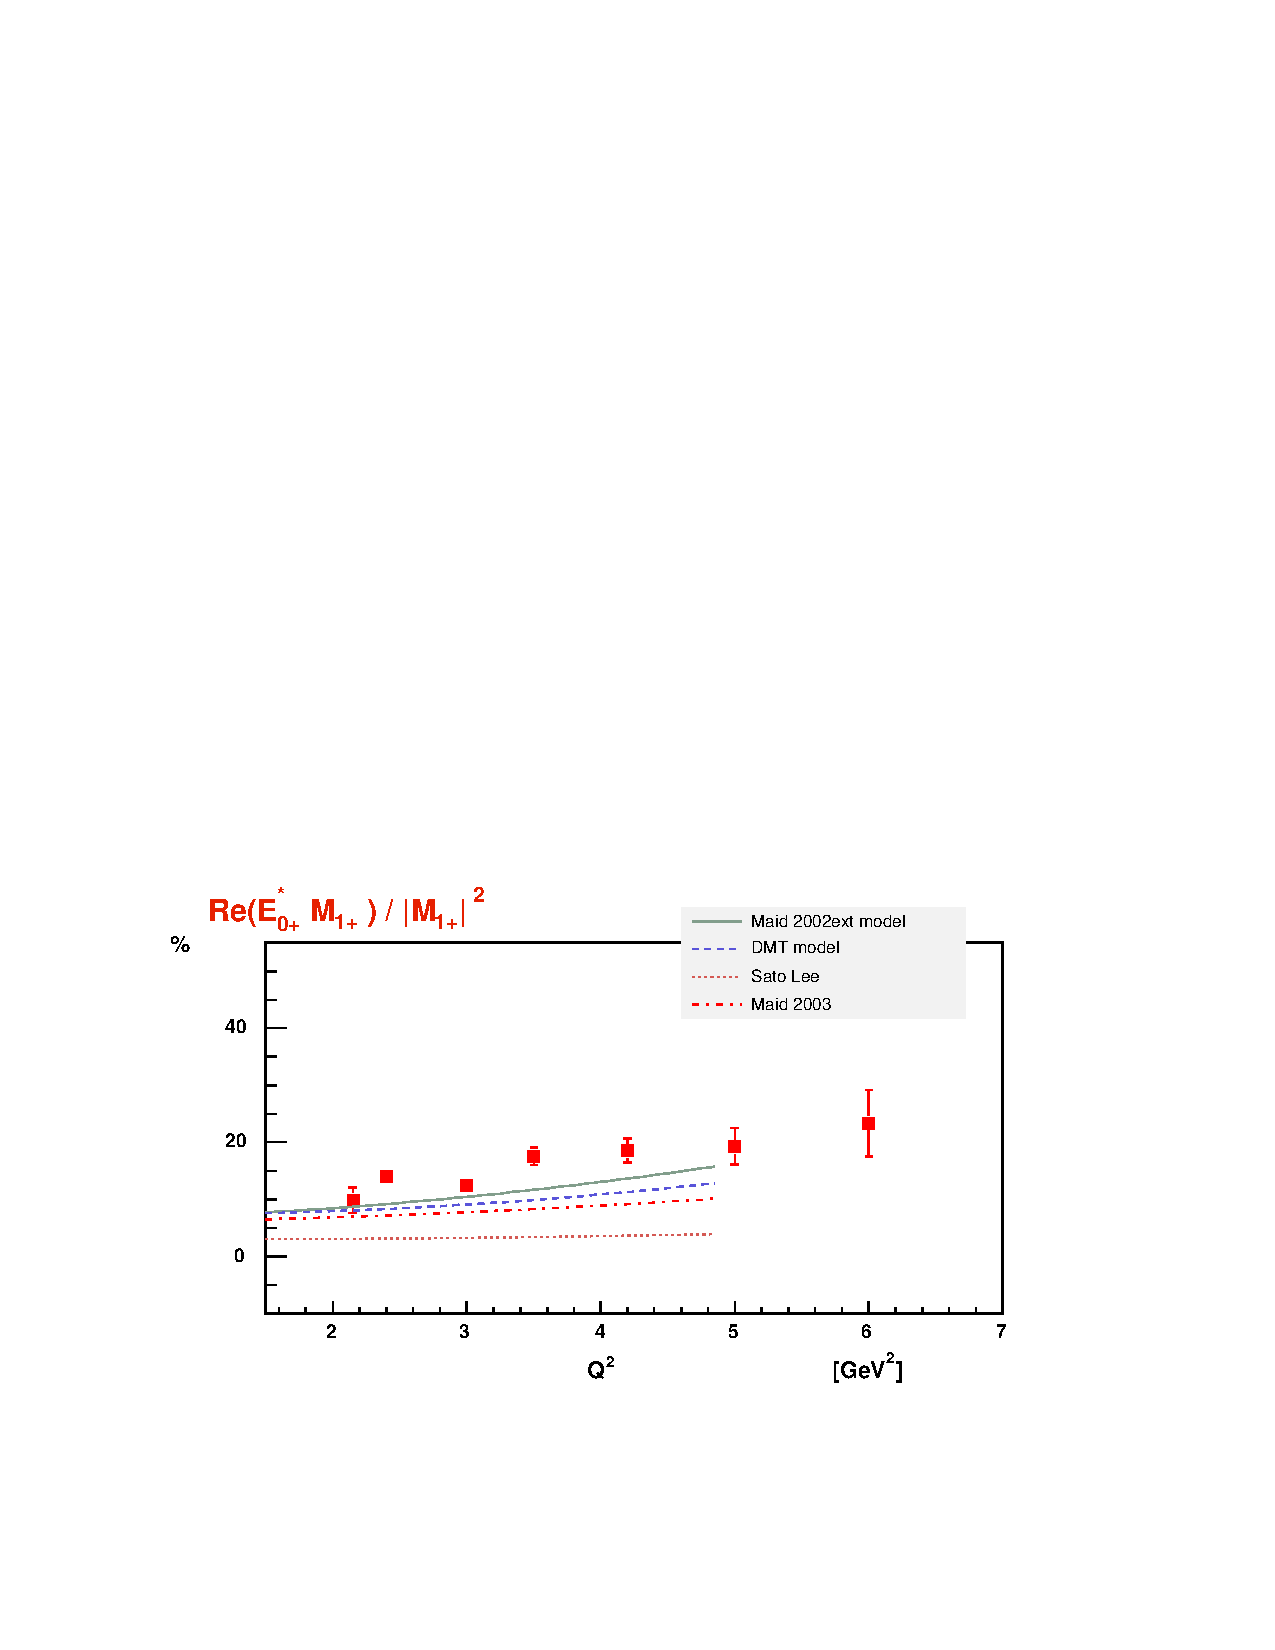
\includegraphics[width = 11cm, bb=30 120 520 400]{analysis/img/E0p} 
 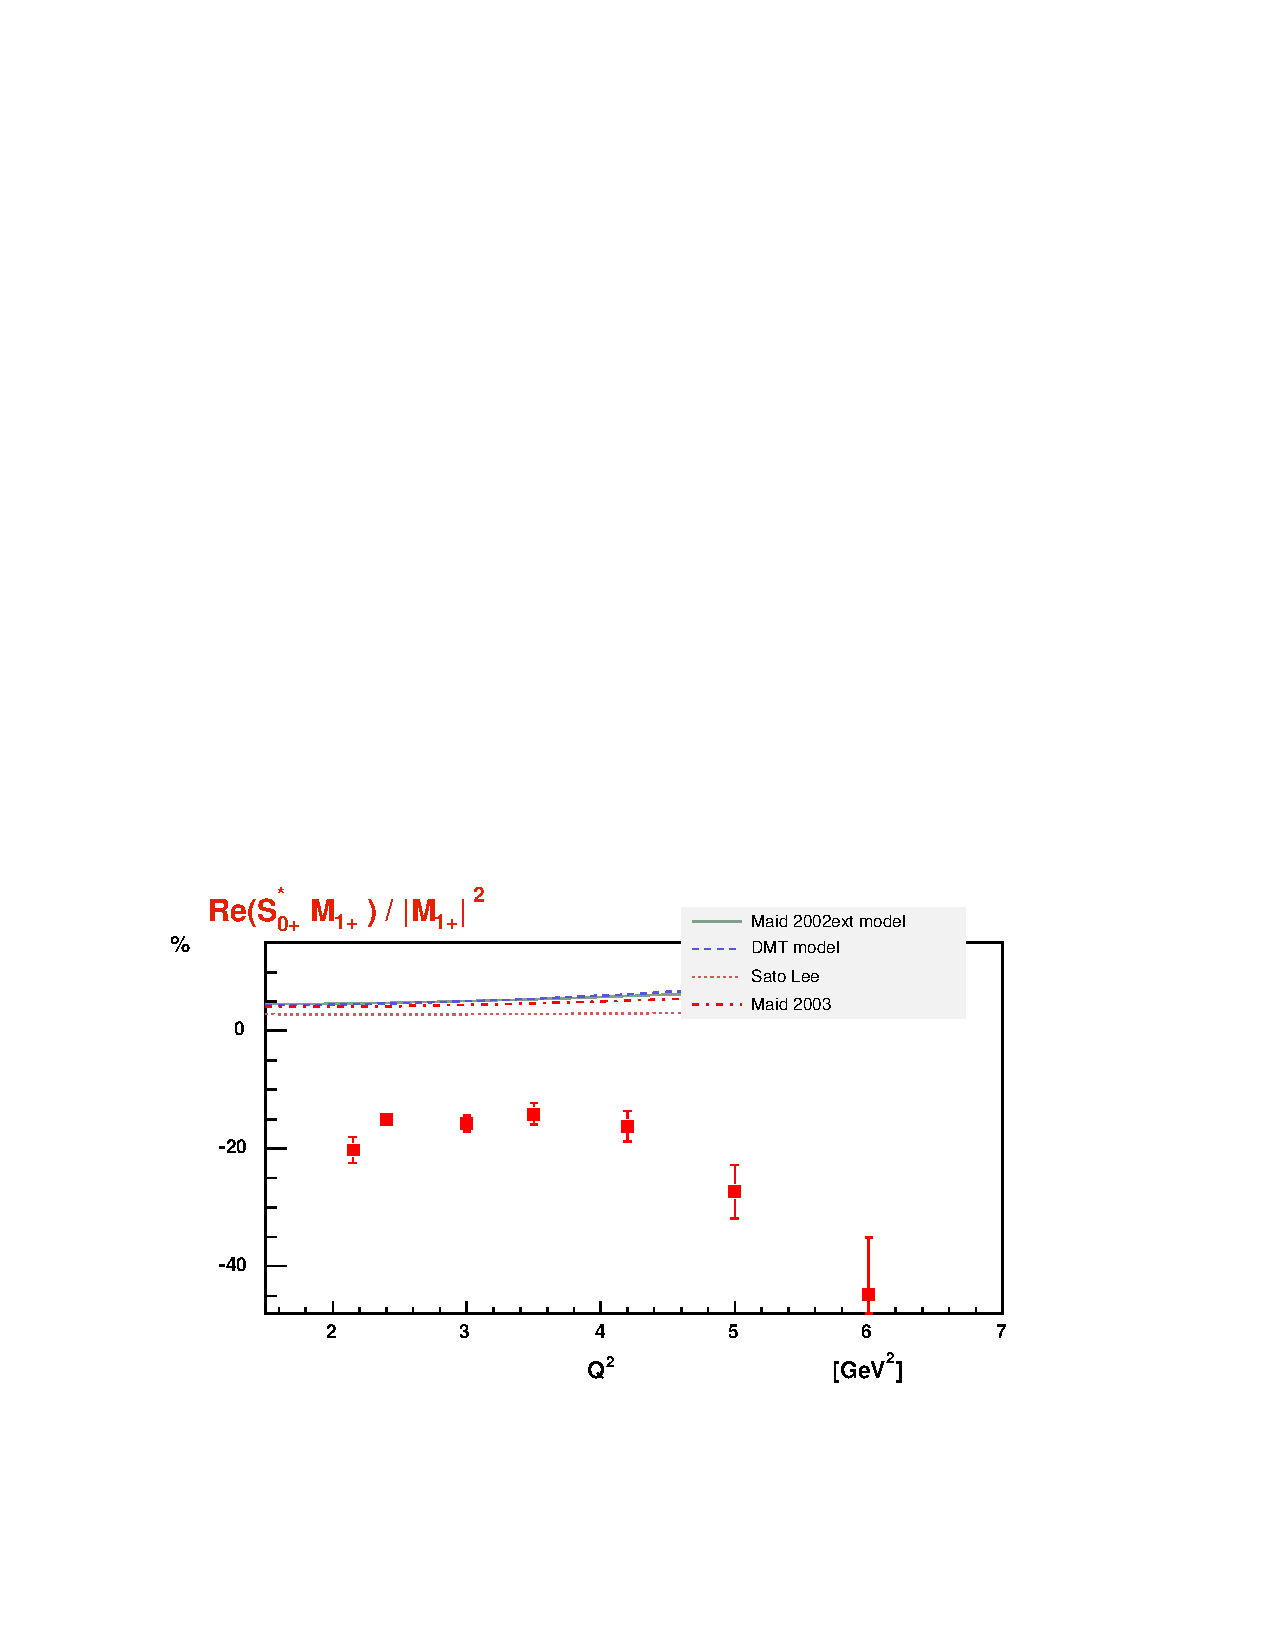
\includegraphics[width = 11cm, bb=30 110 520 400]{analysis/img/S0p} 
  \caption[Amplitudes of $E_{0+}$ and $S_{0+}$]
{  Result for  $E_{0+}$ and $S_{0+}$ as a function of $Q^2$ obtained in the $M_{1+}$ dominance approximation.}
 \label{fig:E0p}
\end{center}
\end{figure}
















